\documentclass{article}
%\documentclass[11pt,letterpaper,twoside,english,final]{article}
\usepackage{graphicx}
\usepackage{caption}
\usepackage{subcaption}
\usepackage{hyperref}
\usepackage{listings}
\usepackage{color}

\definecolor{dkgreen}{rgb}{0,0.6,0}
\definecolor{gray}{rgb}{0.5,0.5,0.5}
\definecolor{mauve}{rgb}{0.58,0,0.82}

\lstset{frame=tb,
  language=Java,
  aboveskip=3mm,
  belowskip=3mm,
  showstringspaces=false,
  columns=flexible,
  basicstyle={\small\ttfamily},
  numbers=none,
  numberstyle=\tiny\color{gray},
  keywordstyle=\color{blue},
  commentstyle=\color{dkgreen},
  stringstyle=\color{mauve},
  breaklines=true,
  breakatwhitespace=true,
  tabsize=3
}

\begin{document}

\section*{Dynamically Extending the Eclipse ICE UI}

This tutorial will show you how to create custom, dynamic UI extensions to
Eclipse ICE.

What you will need for this tutorial:
\begin{itemize}
\item Experience creating Eclipse plugins
\item Experience writing UI code with SWT
\item Experience creating an ICE Item
\end{itemize}

\section{Introduction}

ICE makes some educated guesses based on the type of your components and
information that it can glean from your data to figure out the best way that it
can generate the the UI. However, after you create your first set of Items, you
might find yourself wondering if you can change the way that ICE auto-generates
the UI to better fit your needs. ICE lets you do this by setting the Context of
your Form and Components with the setContext() operation. Setting the context
with a string that is unique to your project will let ICE look up UI extensions
that you create and publish through the Eclipse 4 framework.

There are several important things to consider before you start extending the
UI. First, how much work do you want to do? Some of the UI constructs in ICE
are quick to change, such as EntryComposites for showing Entries, but others,
like GeometryPage and MeshPage, could require significant work because of the
evel graphics involved.

This tutorial will show you how to change two pieces of ICE’s UI: The page for
showing GeometryComponents and an EntryComposite. We will only show you how to
change the GeometryPage, not how to actually generate new 3D graphics. The
source code for this tutorial is in the ICE repo in a project called
org.eclipse.ice.demo.

\section{Create an ICE Item Project}

Use the ICE Item Project Generation Wizard to create a new Item with  a
eometryComponent and a DataComponent with one Entry in the Form. You can copy
the following code into your setupForm() operation:

\begin{lstlisting}[language=java]
@Override
    public void setupForm() {
        form = new Form();

        ioService = getIOService();

        // Create a geometry component
        GeometryComponent geomComp = new GeometryComponent();
        geomComp.setName("Geometry");
        geomComp.setDescription("A geometry");
        geomComp.setContext("demo-geometry");
        geomComp.setGeometry(
                new ShapeController(new ShapeMesh(), new AbstractView()));

        // Create a data component
        DataComponent dataComp = new DataComponent();
        dataComp.setName("Data");
        dataComp.setDescription("Some Data");
        dataComp.setContext("demo");
        // Need to set the id since geomComp is number 1
        dataComp.setId(2);

        // Create an Entry for the data component
        IEntry entry = new StringEntry();
        entry.setName("Data Entry");
        entry.setDescription("An Entry with Important Data");
        entry.setContext("demo-entry");
        // Add the Entry to the data component
        dataComp.addEntry(entry);

        // Add both components to the Form, showing the data component first.
        form.addComponent(dataComp);
        form.addComponent(geomComp);

        // Set the context on the Form
        form.setContext("demo");

        return;
    }
\end{lstlisting}

Note that your import packages lines should look this the following:

\begin{lstlisting}[language=java]
import org.eclipse.core.resources.IFile;
import org.eclipse.core.resources.IProject;
import org.eclipse.core.runtime.CoreException;
import org.eclipse.eavp.viz.service.modeling.AbstractView;
import org.eclipse.eavp.viz.service.modeling.ShapeController;
import org.eclipse.eavp.viz.service.modeling.ShapeMesh;
import org.eclipse.ice.datastructures.entry.IEntry;
import org.eclipse.ice.datastructures.entry.StringEntry;
import org.eclipse.ice.datastructures.form.DataComponent;
import org.eclipse.ice.datastructures.form.Form;
import org.eclipse.ice.datastructures.form.FormStatus;
import org.eclipse.ice.datastructures.form.GeometryComponent;
import org.eclipse.ice.io.serializable.IIOService;
import org.eclipse.ice.io.serializable.IReader;
import org.eclipse.ice.io.serializable.IWriter;
import org.eclipse.ice.item.model.Model;
\end{lstlisting}

You may need to add some of these packages to your Manifest file.

If you have not created an Item in ICE before, please see <the ICE Item
Generation tutorial> to do this.

Add this plugin to the launch configuration for your system, launch ICE and
make sure that you can successfully create a DemoModel Item. You should have
see a Form with two pages as in figures \ref{fig:iceDefaultEntryPage} and
\ref{fig:iceDefaultGeometryPage}.

\begin{figure}[h]
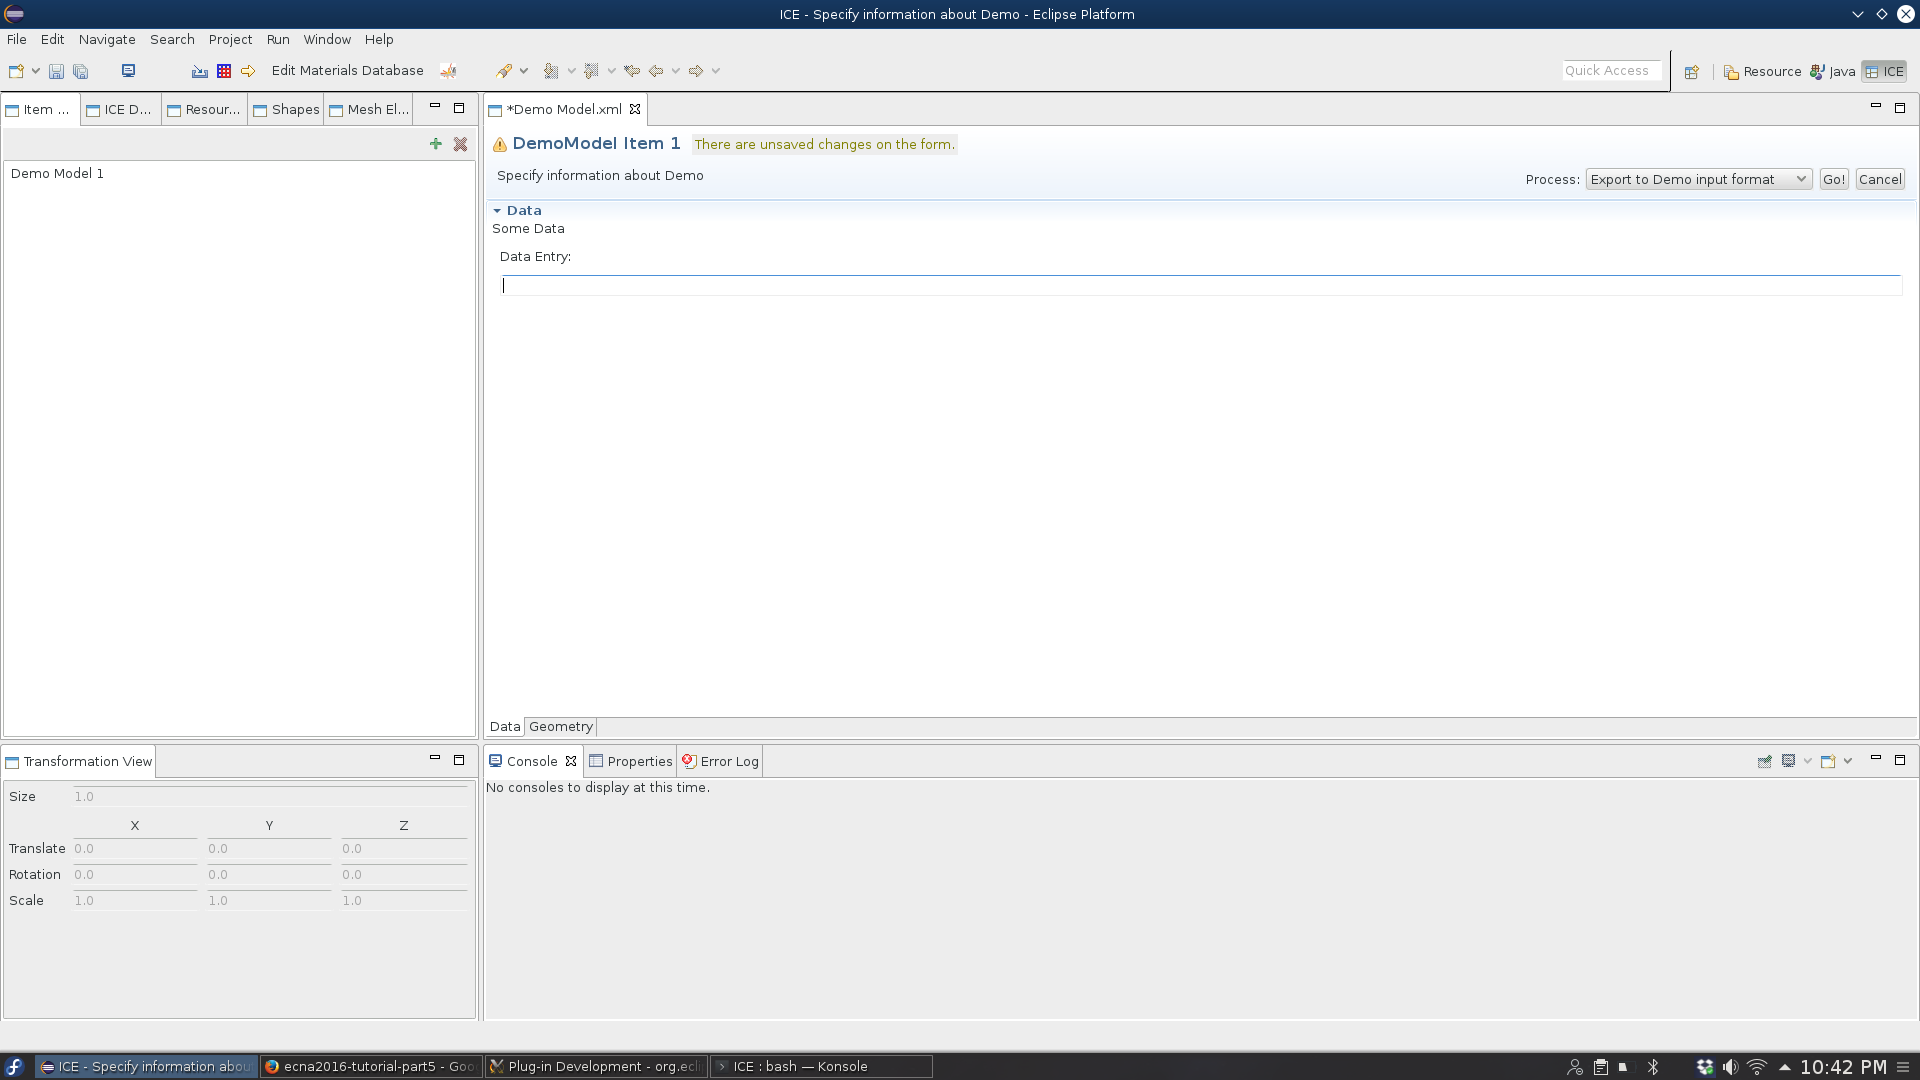
\includegraphics[width=\textwidth]{pics/dynamicUI_defaultEntryPage.png}
\caption{Default Entry Composite on a Form}
\label{fig:iceDefaultEntryPage}
\end{figure}

\begin{figure}[h]
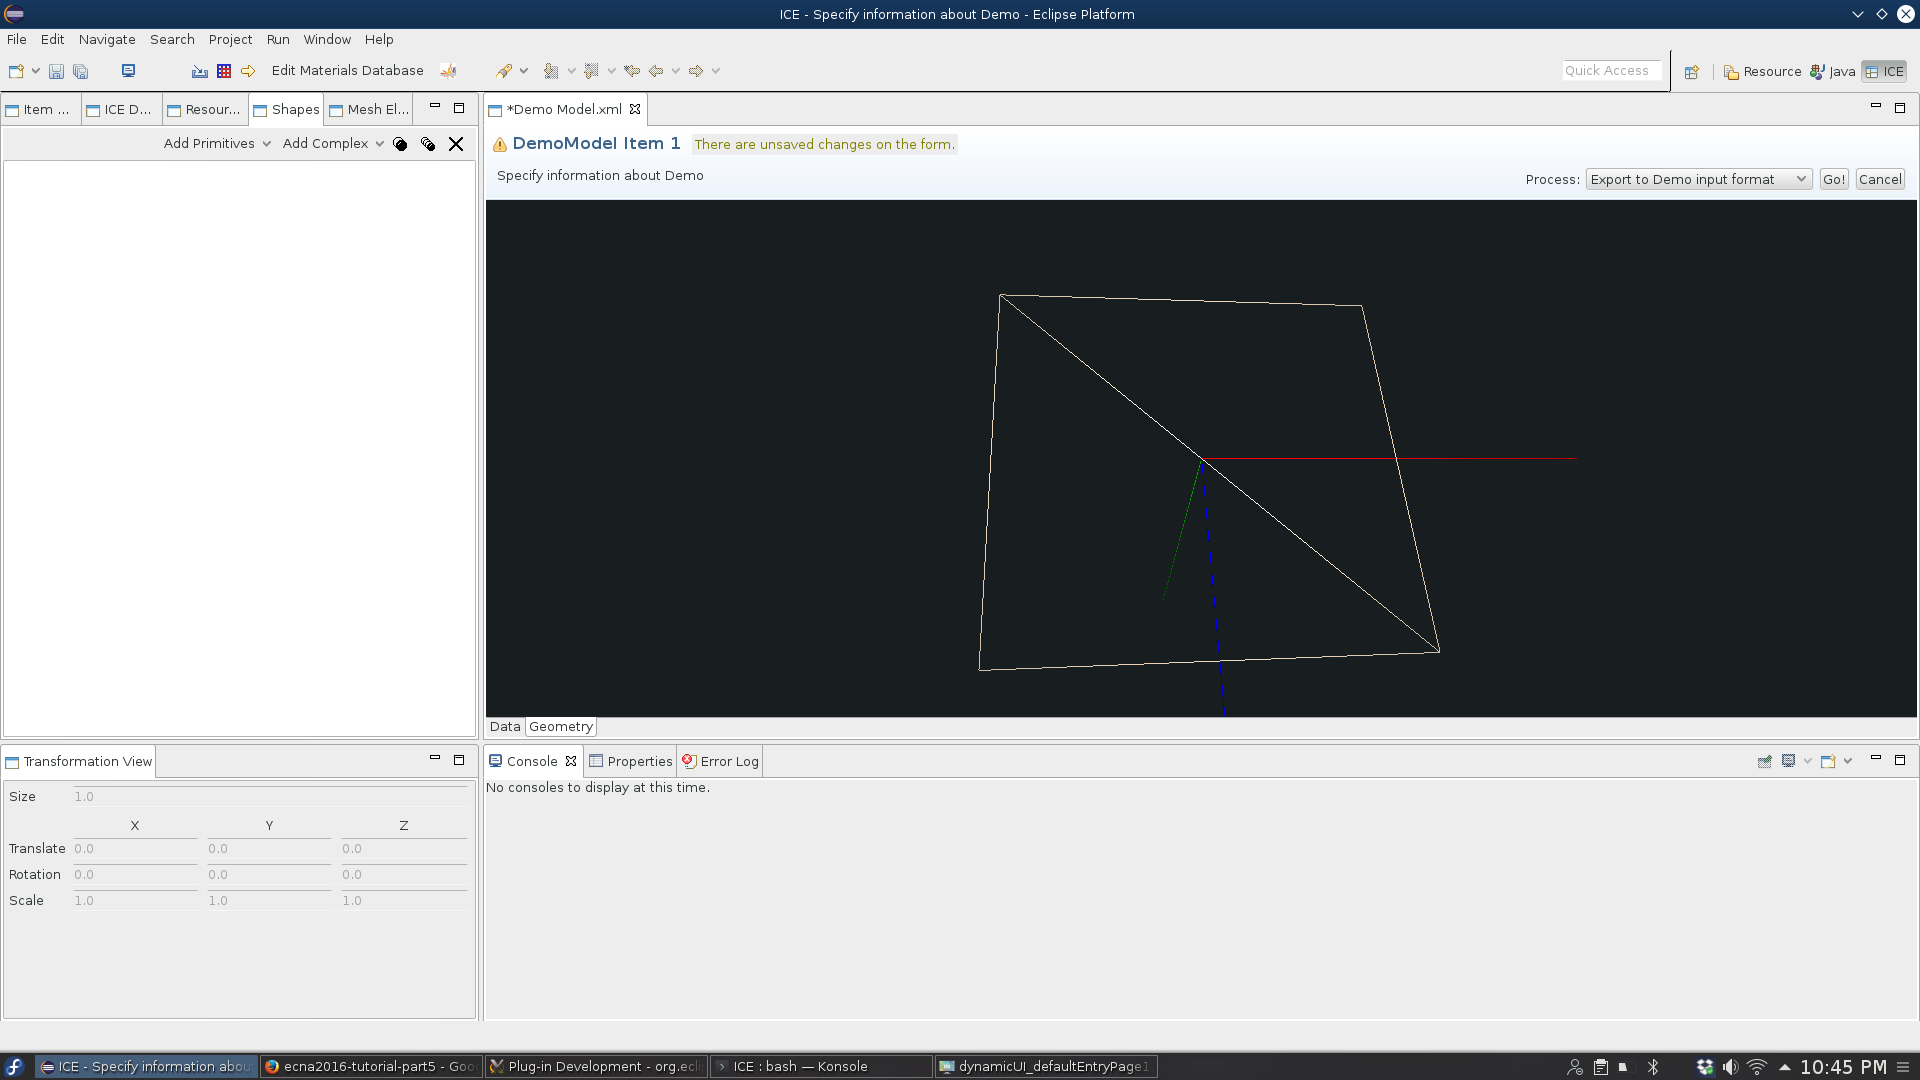
\includegraphics[width=\textwidth]{pics/dynamicUI_defaultGeometryPage.png}
\caption{Default Geometry Page}
\label{fig:iceDefaultGeometryPage}
\end{figure}

The rest of the tutorial will look at replacing the routine that draws the
Entry on the first page and the entire Geometry Page with your own custom page.
You won’t have to make any additional changes to your Item (assuming it works
as shown above). Note that in the code above we need to use different context
names for the Entry and the GeometryComponent so that the context can uniquely
identify the routines that draw each.

\section{Create an IPageProvider and IPageFactory}

We will replace the Geometry Page first. Create a new package.This requires two
pieces to properly locate your Page, through your IPageFactory, and to draw
your Page, through you IPageProvider.

Start by adding the following packages to your import packages block in your
Manifest file:
\begin{itemize}
  \item org.eclipse.ice.client.widgets.providers
  \item org.eclipse.ice.client.widgets.providers.Default
  \item org.eclipse.ui.forms
  \item org.eclipse.ui.forms.editor
  \item org.eclipse.ui.forms.widgets
  \item org.eclipse.e4.core.contexts
  \item org.eclipse.e4.core.di
  \item org.eclipse.e4.ui.model.application
  \item org.eclipse.e4.ui.model.application.ui
\end{itemize}

Create a class that implements IPageProvider and copy the following code into
it:

\begin{lstlisting}[language=java]
public class DemoGeometryPageProvider implements IPageProvider {

    @Override
    public String getName() {
        // TODO Auto-generated method stub
        return "demo";
    }

    @Override
    public ArrayList<IFormPage> getPages(FormEditor formEditor,
            ArrayList<Component> components) {

        ArrayList<IFormPage> pages = new ArrayList<IFormPage>();
        // Get the GeometryComponent and create the GeometryPage.
        if (!(components.isEmpty())) {
            GeometryComponent geometryComponent = (GeometryComponent) (components
                    .get(0));

            if (geometryComponent != null) {

                // Make the GeometryPage
                DemoGeometryPage geometryPage = new DemoGeometryPage(formEditor,
                        "GPid", geometryComponent.getName());

                // No need to set the geometry component for the demo, but
                // something like would be necessary in a real application.
                // geometryPage.setGeometry(geometryComponent);

                // Add the page
                pages.add(geometryPage);
            }

        }

        return pages;
    }

}
\end{lstlisting}

This class will provide your page to the platform. We need a second class that
actually draws the content on the Geometry page. We will create a third class
here, for convenience, that inherits from ICE’s ICEFormPage base class to act
as the GeometryPage. We don’t actually need to show the content of the Geometry
component for now because we just want to show that we can change the page. So,
create your class and copy the following code into it to just show a label in
place of the original 3D editor:

\begin{lstlisting}[language=java]
public class DemoGeometryPage extends ICEFormPage {

    public DemoGeometryPage(FormEditor editor, String id, String title) {
        super(editor, id, title);
        // TODO Auto-generated constructor stub
    }

    /**
     * <p>
     * Provides the page with the geometryApplication's information to display
     * geometry.
     * </p>
     *
     * @param managedForm
     *            the managed form that handles the page
     */
    @Override
    public void createFormContent(IManagedForm managedForm) {

        // Local Declarations
        final ScrolledForm form = managedForm.getForm();
        GridLayout layout = new GridLayout();

        // Setup the layout and layout data
        layout.numColumns = 1;
        form.getBody().setLayoutData(
                new GridData(SWT.FILL, SWT.FILL, true, true, 1, 1));
        form.getBody().setLayout(new FillLayout());

        // Just create some text and say hello
        Label geometryText = new Label(form.getBody(), SWT.FLAT);
        geometryText.setText("Draw something based on the geometry.");

        return;

    }

}
\end{lstlisting}

\section{Create a new IEntryComposite}

Individual Entry’s that ICE draws can be extended in the same way. First,
create a subclass of AbstractEntryComposite that implements render and copy the
following code into it:

\begin{lstlisting}[language=java]
public class DemoEntryComposite extends AbstractEntryComposite {

    public DemoEntryComposite(Composite parent, IEntry refEntry, int style) {
        super(parent, refEntry, style);
    }

    @Override
    public void render() {

        Button button = new Button(this, SWT.PUSH);
        button.setText("My button");

        Label label = new Label(this, SWT.FLAT);
        label.setText(super.getEntry().getValue() + " in new Entry widget.");
        setLayout(new FillLayout());
        this.layout();

        return;
    }

}
\end{lstlisting}

Next, create a provider to publish your Entry Composite to the platform and
copy the following code into it:

\begin{lstlisting}[language=java]
public class DemoEntryCompositeProvider implements IEntryCompositeProvider {

    @Override
    public String getName() {
        // TODO Auto-generated method stub
        return "demo-entry";
    }

    @Override
    public IEntryComposite getEntryComposite(Composite parent, IEntry entry,
            int style, FormToolkit toolKit) {
        // TODO Auto-generated method stub
        return new DemoEntryComposite(parent, entry, style);
    }

}
\end{lstlisting}

\section{Publishing through the e4 extension point}

The most common way to publish these extensions to the platform is to create an
extension at the org.eclipse.e4.workbench.model extension point. You can do this
by creating an executable processor. Create a new class and add the following
code:

\begin{lstlisting}[language=java]

public class DemoWidgetsProcessor {

	/**
	 * This operation executes the instructions required to register the demo
	 * widgets with the e4 workbench.
	 * 
	 * @param context
	 *            The e4 context
	 * @param app
	 *            the model application
	 */
	@Execute
	public void execute(IEclipseContext context, MApplication app) {

		// Add the geometry provider
		IPageProvider provider = ContextInjectionFactory
				.make(DemoGeometryPageProvider.class, context);
		context.set("demo-geometry", provider);

		// Add the EntryComposite provider
		IEntryCompositeProvider compProvider = ContextInjectionFactory
				.make(DemoEntryCompositeProvider.class, context);
		context.set("demo-entry", compProvider);

	}

}

\end{lstlisting}

Next, either create an extension point graphically or add the following code to
your plugin.xml file:

\begin{lstlisting}[language=java]

   <extension
         id="org.eclipse.ice.demo.ui.processor"
         name="ICE Demo UI Processor"
         point="org.eclipse.e4.workbench.model">
      <processor
            apply="always"
            beforefragment="true"
            class="org.eclipse.ice.demo.ui.DemoWidgetsProcessor">
      </processor>
   </extension>

\end{lstlisting}

Your extensions will now be available in the workbench. Your entry composite is
should look like fig. \ref{fig:iceDemoEntryComposite}.

\begin{figure}[h]
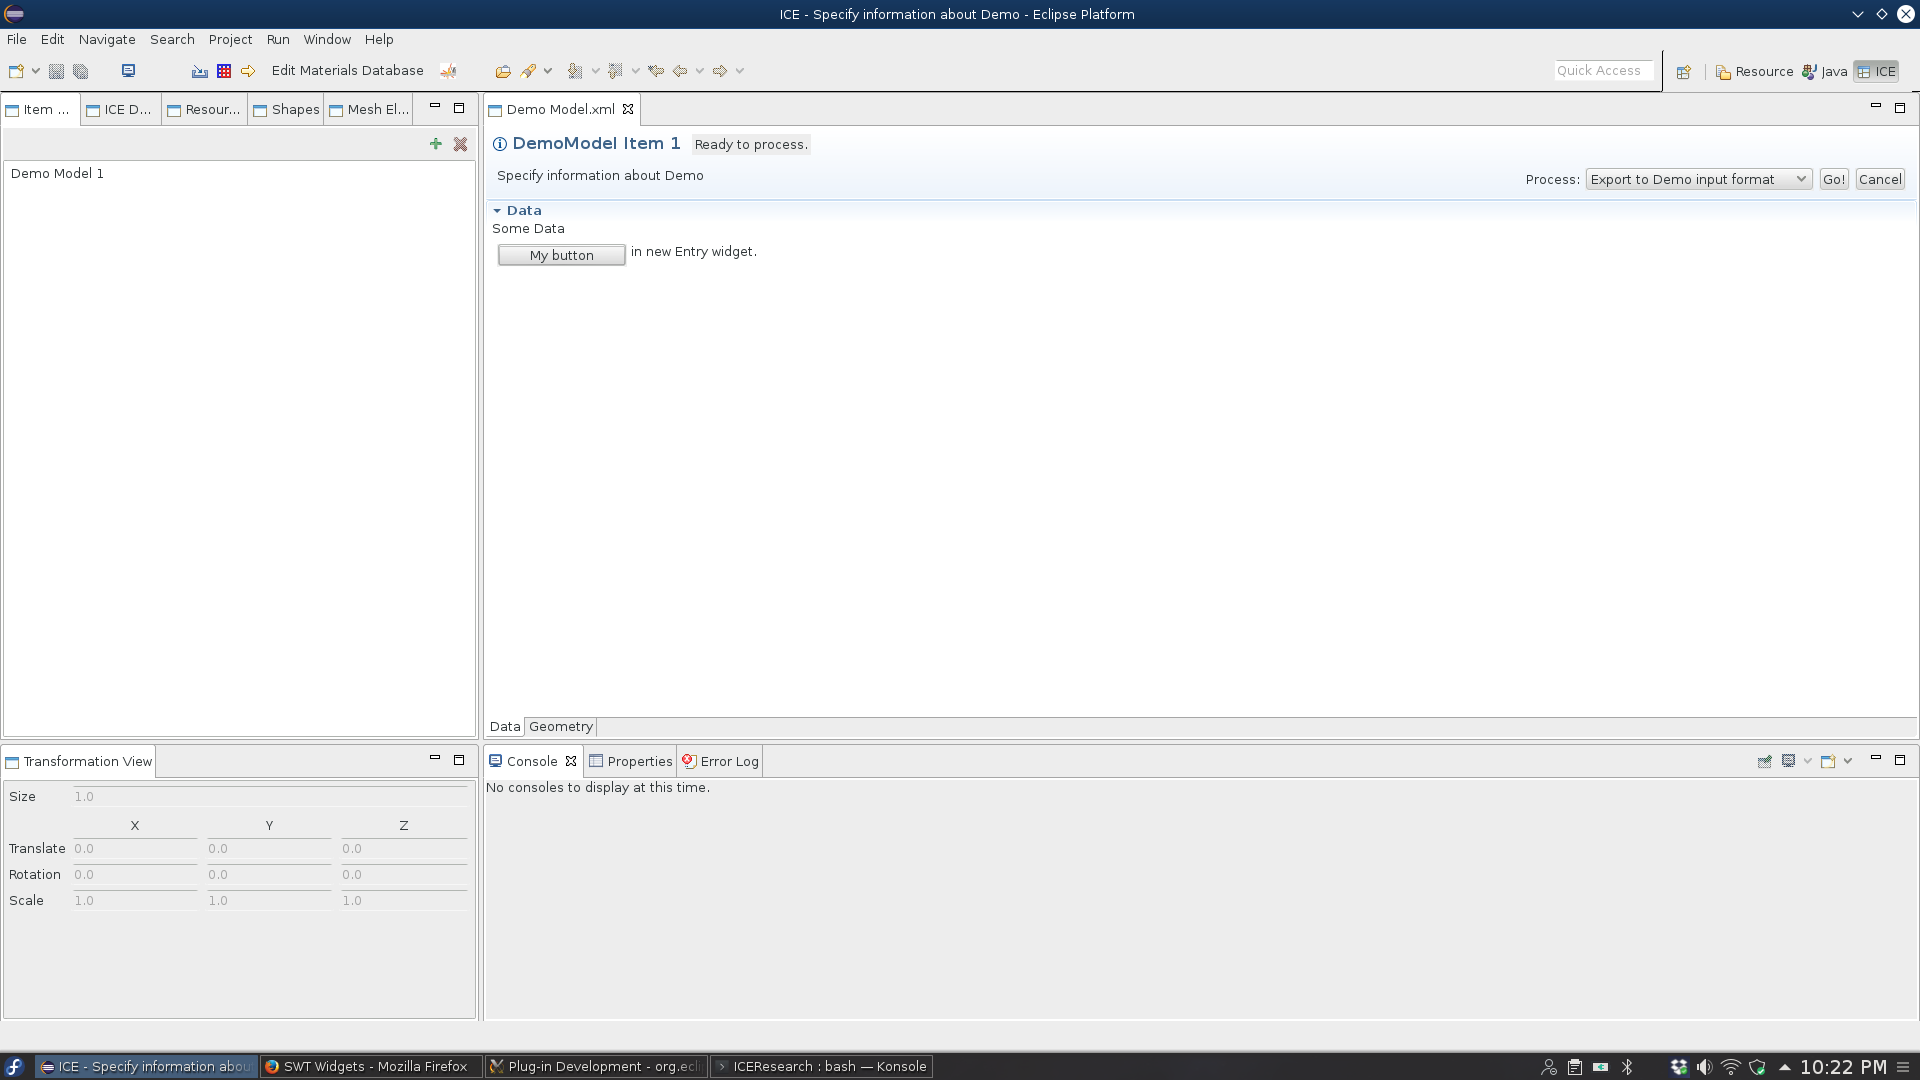
\includegraphics[width=\textwidth]{pics/dynamicUI_demoEntryComposite.png}
\caption{Updated Entry Widget}
\label{fig:iceDemoEntryComposite}
\end{figure}

You geometry component should look like fig. \ref{fig:iceDemoGeometryPage}.

\begin{figure}[h]
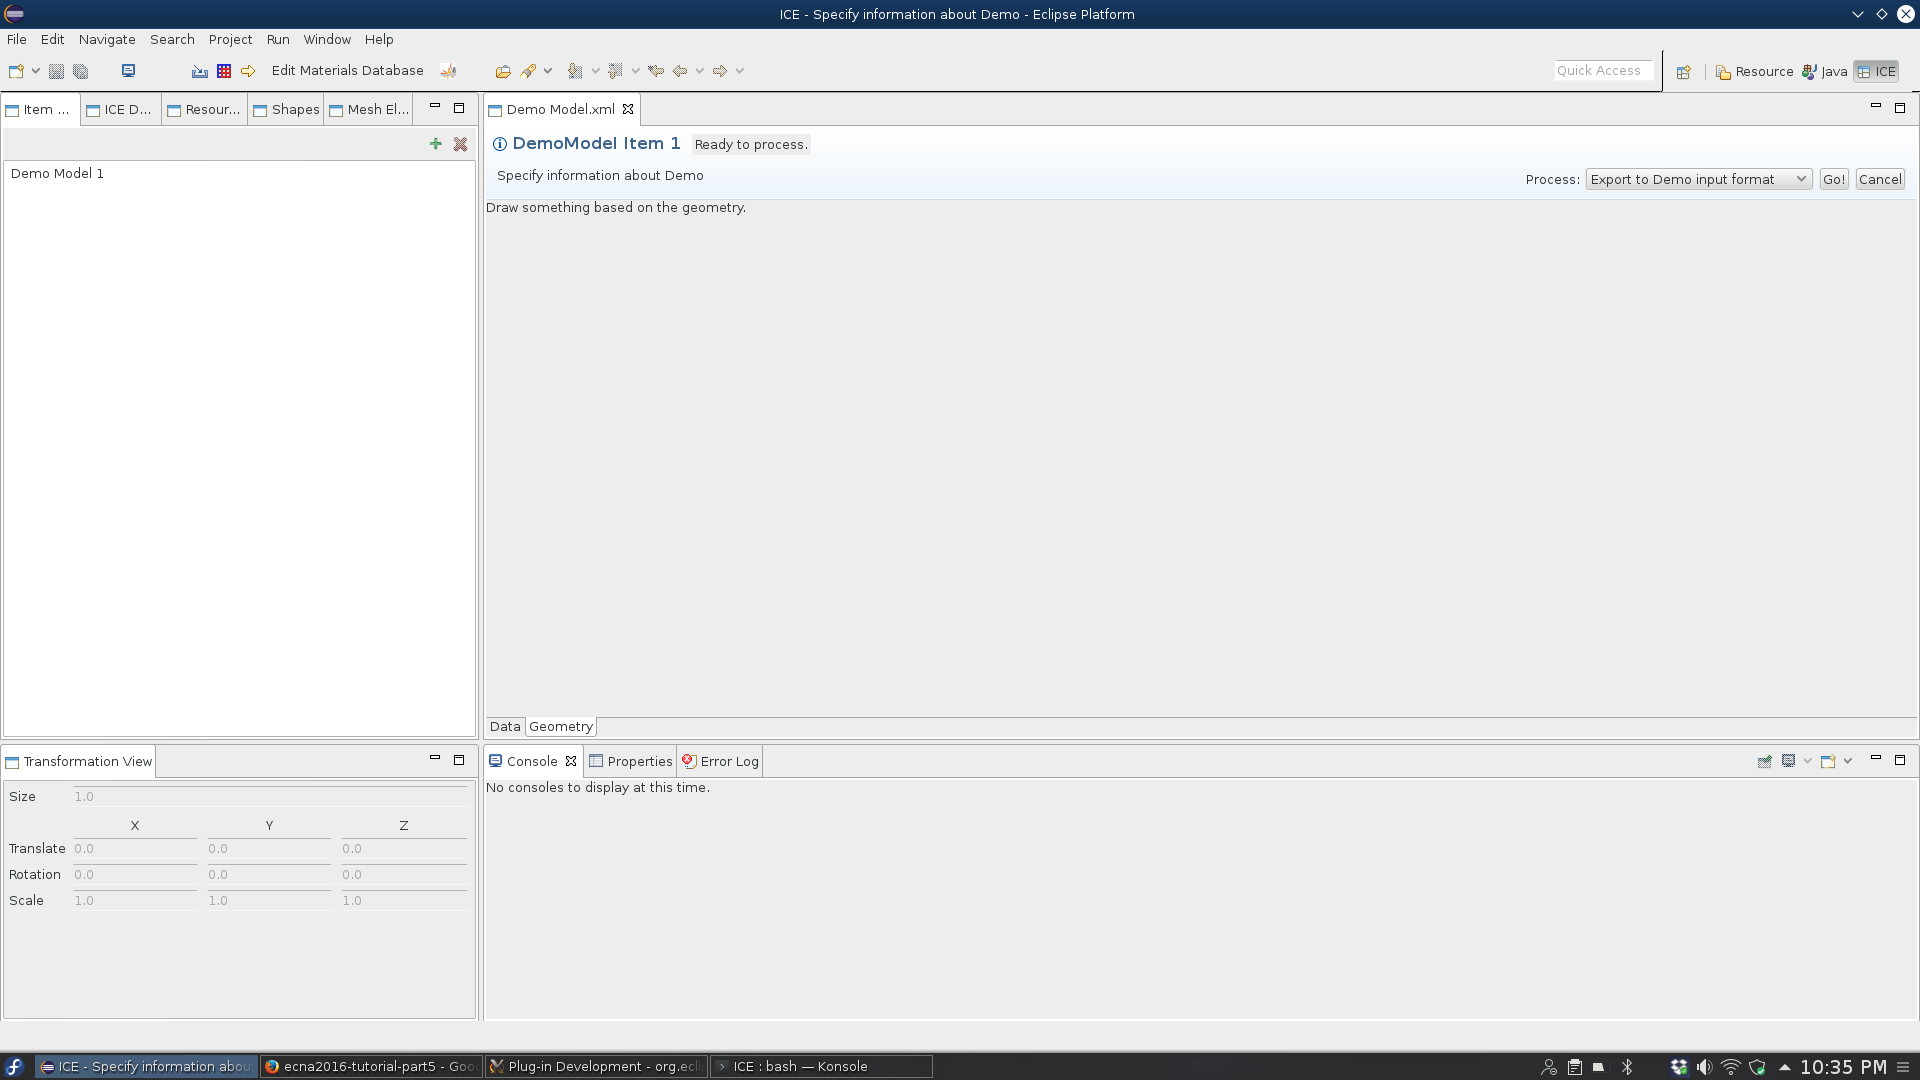
\includegraphics[width=\textwidth]{pics/dynamicUI_demoGeometryPage.png}
\caption{The updated Geometry page.}
\label{fig:iceDemoGeometryPage}
\end{figure}

\section{Publishing through Context Functions}

Make sure to check “Activate this plug-in when one of its classes loaded.” in
your MANIFEST.mf file.

You can alternatively publish your new extensions to the OSGI framework so that
they can be dynamically injected into the ICE’s UI code. These extensions are
registered as standalone services that are dynamically located at runtime based
on the context name that you specified in your data structures. The benefit of
this method over the extension point is that it can be used to dynamically
update based on the \textit{present} context of the UI, not the initial
context. This means that in addition to the type of data structure involved the
UI can be tailored based on the particular area of the workbench where it would
be drawn and the current runtime state.

Create a new context function for your IEntryComposite. You should create a
subclass of ContextFunction with the following code:

\begin{lstlisting}[language=java]
public class DemoEntryCompositeContextFunction extends ContextFunction {

    @Override
    public Object compute(IEclipseContext context, String contextKey) {
        IEntryCompositeProvider provider = ContextInjectionFactory
                .make(DemoEntryCompositeProvider.class, context);
        // add the new object to the application context
        MApplication application = context.get(MApplication.class);
        IEclipseContext ctx = application.getContext();
        ctx.set(IEntryCompositeProvider.class, provider);
        return provider;
    }

}
\end{lstlisting}

Create an OSGI component with the following contents:

\begin{lstlisting}[language=xml]
<?xml version="1.0" encoding="UTF-8"?>
<scr:component xmlns:scr="http://www.osgi.org/xmlns/scr/v1.1.0"
name="org.eclipse.ice.demo.entry"> <implementation
   class="org.ecli pse.ice.demo.ui.DemoEntryCompositeContextFunction"/>
   <property name="service.context.key" type="String" value="demo-entry"/>
   <service> <provide
   interface="org.eclipse.e4.core.contexts.IContextFunction"/> </service>
</scr:component>
\end{lstlisting}

Now, create a context function for your Geometry Page. You should create a
subclass of ContextFunction with the following code:

\begin{lstlisting}[language=java]
public class DemoGeometryPageContextFunction extends ContextFunction {

    @Override
    public Object compute(IEclipseContext context, String contextKey) {
        IPageProvider provider = ContextInjectionFactory
                .make(DemoGeometryPageProvider.class, context);
        // add the new object to the application context
        MApplication application = context.get(MApplication.class);
        IEclipseContext ctx = application.getContext();
        ctx.set(IPageProvider.class, provider);
        return provider;
    }

}
\end{lstlisting}

and an OSGI component with the following contents:

\begin{lstlisting}[language=xml]
<?xml version="1.0" encoding="UTF-8"?>
<scr:component xmlns:scr="http://www.osgi.org/xmlns/scr/v1.1.0"
name="org.eclipse.ice.demo.geometry.page"> <implementation
class="org.eclipse.ice.demo.ui.DemoGeometryPageContextFunction"/> <property
name="service.context.key" type="String" value="demo-geometry"/> <service>
      <provide interface="org.eclipse.e4.core.contexts.IContextFunction"/>
   </service>
</scr:component>
\end{lstlisting}

\section{Replacing the whole Page Factory}

If you want to replace the way that all pages in ICE are drawn, you can replace
the entire Page Factory.  Create a new class in your package that inherits from
DefaultPageFactory, which will save you some work over implementing an entire
new factory from scratch. See fig. \ref{fig:icegeometryPageClass}.

\begin{figure}[h]
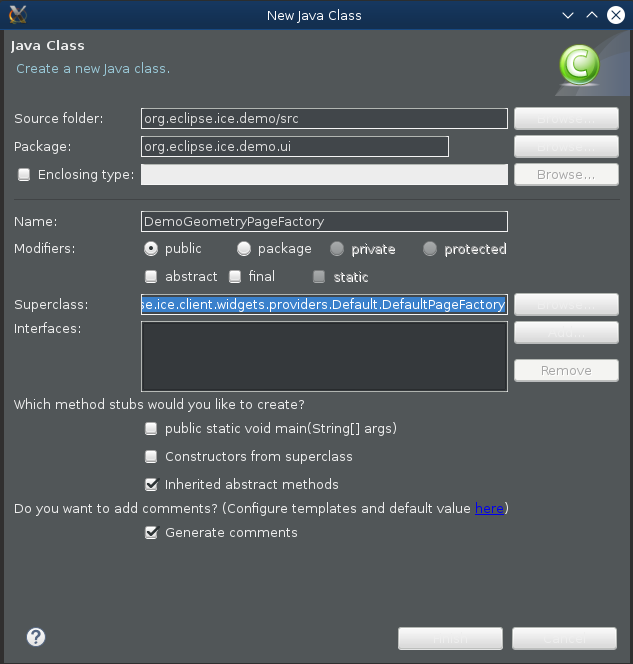
\includegraphics[width=\textwidth]{pics/dynamicUI_geometryPageClass.png}
\caption{Generating the Page Factory class.}
\label{fig:icegeometryPageClass}
\end{figure}

Copy the following code into your new subclass:

\begin{lstlisting}[language=java]
public class DemoGeometryPageFactory extends DefaultPageFactory {

    @Override
    public ArrayList<IFormPage> getGeometryComponentPages(FormEditor editor,
            ArrayList<Component> components) {
        DemoGeometryPageProvider pageProvider = new DemoGeometryPageProvider();
        return pageProvider.getPages(editor, components);
    }
}
\end{lstlisting}

This will now build on your previous DemoGeometryPageProvider to provide it to
the framework through a factory. You can override other operations to provide
access to other custom pages. This method may be more efficient than creating
separate page extension for each page type. To publish this to the platform,
create a Context Function with the following code:

\begin{lstlisting}[language=java]
public class DemoGeometryPageFactoryContextFunction extends ContextFunction {

    @Override
    public Object compute(IEclipseContext context, String contextKey) {
        IPageFactory factory = ContextInjectionFactory
                .make(DemoGeometryPageFactory.class, context);
        // add the new object to the application context
        MApplication application = context.get(MApplication.class);
        IEclipseContext ctx = application.getContext();
        ctx.set(IPageFactory.class, factory);
        return factory;
    }

}
\end{lstlisting}

Your OSGI component should be published as such:

\begin{lstlisting}[language=xml]
<?xml version="1.0" encoding="UTF-8"?>
<scr:component xmlns:scr="http://www.osgi.org/xmlns/scr/v1.1.0"
name="org.eclipse.ice.demo.factory"> <implementation
class="org.eclipse.ice.demo.ui.DemoGeometryPageFactoryContextFunction"/>
<property name="service.context.key" type="String" value="demo"/> <service>
      <provide interface="org.eclipse.e4.core.contexts.IContextFunction"/>
   </service>
</scr:component>
\end{lstlisting}

and your MANIFEST.mf file should contain:

\begin{lstlisting}[language=xml]
Service-Component: OSGI-INF/*.xml
\end{lstlisting}

\end{document}